\documentclass[notes,11pt, aspectratio=169]{beamer}

\usepackage{pgfpages}
% These slides also contain speaker notes. You can print just the slides,
% just the notes, or both, depending on the setting below. Comment out the want
% you want.
\setbeameroption{hide notes} % Only slide
%\setbeameroption{show only notes} % Only notes
%\setbeameroption{show notes on second screen=right} % Both
\usepackage{csquotes}
\usepackage{hyperref}
\usepackage{helvet}
\usepackage[default]{lato}
\usepackage{array}
\usepackage{tgbonum}
\usepackage{tikz}
\setbeamertemplate{note page}{\pagecolor{yellow!5}\insertnote}
\usetikzlibrary{positioning}
\usetikzlibrary{snakes}
\usetikzlibrary{calc}
\usetikzlibrary{arrows}
\usetikzlibrary{decorations.markings}
\usetikzlibrary{shapes.misc}
\usetikzlibrary{matrix,shapes,arrows,fit,tikzmark}
\usepackage{amsmath}
\usepackage{mathpazo}
\usepackage{hyperref}
\usepackage{lipsum}
\usepackage{multimedia}
\usepackage{multirow}
\usepackage{graphicx}
\usepackage{dcolumn}
\usepackage{bbm}
\usepackage{xcolor}
\usepackage{changepage}
\usepackage{appendixnumberbeamer}
\newcommand{\beginbackup}{
   \newcounter{framenumbervorappendix}
   \setcounter{framenumbervorappendix}{\value{framenumber}}
   \setbeamertemplate{footline}
   {
     \leavevmode%
     \hline
     box{%
       \begin{beamercolorbox}[wd=\paperwidth,ht=2.25ex,dp=1ex,right]{footlinecolor}%
%         \insertframenumber  \hspace*{2ex} 
       \end{beamercolorbox}}%
     \vskip0pt%
   }
 }
\newcommand{\backupend}{
   \addtocounter{framenumbervorappendix}{-\value{framenumber}}
   \addtocounter{framenumber}{\value{framenumbervorappendix}} 
}


\usepackage{graphicx}
\usepackage[space]{grffile}
\usepackage{booktabs}
\newcommand\independent{\protect\mathpalette{\protect\independenT}{\perp}}
\def\independenT#1#2{\mathrel{\rlap{$#1#2$}\mkern2mu{#1#2}}}
\DeclareMathOperator{\Supp}{Supp}

% These are my colors -- there are many like them, but these ones are mine.
\definecolor{blue}{RGB}{0,115,177}
\definecolor{red}{RGB}{217,90,0}
\definecolor{yellow}{RGB}{239,227,63}
\definecolor{green}{RGB}{0,159,111}

\hypersetup{
  colorlinks=false,
  linkbordercolor = {white},
  linkcolor = {blue}
}


%% I use a beige off white for my background
\definecolor{MyBackground}{RGB}{250,250,218}

%% Uncomment this if you want to change the background color to something else
%\setbeamercolor{background canvas}{bg=MyBackground}

%% Change the bg color to adjust your transition slide background color!
\newenvironment{transitionframe}{
  \setbeamercolor{background canvas}{bg=yellow}
  \begin{frame}}{
    \end{frame}
}

\DeclareFontFamily{U}{skulls}{}
\DeclareFontShape{U}{skulls}{m}{n}{ <-> skull }{}
\newcommand{\skull}{\text{\usefont{U}{skulls}{m}{n}\symbol{'101}}}

\setbeamercolor{frametitle}{fg=blue}
\setbeamercolor{title}{fg=black}
\setbeamertemplate{footline}[frame number]
\setbeamertemplate{navigation symbols}{} 
\setbeamertemplate{itemize items}{-}
\setbeamercolor{itemize item}{fg=blue}
\setbeamercolor{itemize subitem}{fg=blue}
\setbeamercolor{enumerate item}{fg=blue}
\setbeamercolor{enumerate subitem}{fg=blue}
\setbeamercolor{button}{bg=MyBackground,fg=blue,}


\setbeamercolor{section in toc}{fg=blue}
\setbeamercolor{subsection in toc}{fg=red}
\setbeamersize{text margin left=1em,text margin right=1em} 

\newenvironment{wideitemize}{\itemize\addtolength{\itemsep}{10pt}}{\enditemize}

\usepackage{environ}
\NewEnviron{videoframe}[1]{
  \begin{frame}
    \vspace{-8pt}
    \begin{columns}[onlytextwidth, T] % align columns
      \begin{column}{.70\textwidth}
        \begin{minipage}[t][\textheight][t]
          {\dimexpr\textwidth}
          \vspace{8pt}
          \hspace{4pt} {\Large \sc \textcolor{blue}{#1}}
          \vspace{8pt}
          
          \BODY
        \end{minipage}
      \end{column}%
      \hfill%
      \begin{column}{.38\textwidth}
        \colorbox{green!20}{\begin{minipage}[t][1.2\textheight][t]
            {\dimexpr\textwidth}
            Face goes here
          \end{minipage}}
      \end{column}%
    \end{columns}
  \end{frame}
}

\title[]{\textcolor{blue}{Causal Data Analysis and Difference-in-Differences}}
\subtitle[]{\textcolor{blue}{A Short Course}}

\author[DH]{Daniel Halvarsson}

\institute{The Ratio Institute, Stockholm\\
\vspace{0.2cm}
 \href{daniel.halvarsson@ratio.se}{daniel.halvarsson@ratio.se}}

\date{}

\begin{document}
%%% TIKZ STUFF
\tikzset{   
        every picture/.style={remember picture,baseline},
        every node/.style={anchor=base,align=center,outer sep=1.5pt},
        every path/.style={thick},
        }
\newcommand\marktopleft[1]{%
    \tikz[overlay,remember picture] 
        \node (marker-#1-a) at (-.3em,.3em) {};%
}
\newcommand\markbottomright[2]{%
    \tikz[overlay,remember picture] 
        \node (marker-#1-b) at (0em,0em) {};%
}
\tikzstyle{every picture}+=[remember picture] 
\tikzstyle{mybox} =[draw=black, very thick, rectangle, inner sep=10pt, inner ysep=20pt]
\tikzstyle{fancytitle} =[draw=black,fill=red, text=white]

% Title Slide
\begin{frame}
\maketitle
\end{frame}

\begin{frame}{What we will cover:}
\begin{enumerate}
\item Causality
\item Treatment effects 
\item *Basics of $2\times 2$ Difference-in-Difference
\item *Difference-in-Difference via regression analysis
\item Understanding the parallel trends assumption
\item *Evaluating research design (testing pretreatment trends and placebo tests)
\item *Dynamic Difference-in-Difference with multiple time periods
\item *Difference-in-Difference with a roll-out design 
\end{enumerate}
\vspace{0.5cm}
Topics with an * includes a step-by-step coding exercise where you are invited to follow along in Stata. 
\end{frame} 

\begin{frame}{About the course material: Some house keeping}
\begin{itemize}
    \item Data, Stata code, lecture material, and home assignment can all be accessed at 
    \href{https://github.com/DanielHalvarsson/IntroductionDiD/}{\textcolor{blue}{https://github.com/DanielHalvarsson/IntroductionDiD/}}

    \item Much of this course is based on the book "The Effect" by Nick Huntington-Klein, which provides an excellt resource for not just Difference-in-Difference, but empirical research techniques and methods in general.

    \item The Effect is open source and can be freely accessed from 
    \href{https://theeffectbook.net/}{\textcolor{blue}{https://theeffectbook.net/}}
\end{itemize}
\end{frame} 


\begin{frame}{Why are we interested in difference-in-difference?}
    \begin{itemize}
        \item Because we want to understand the causal effect of some \textbf{treatment} e.g. a policy across different groups.
        \item What is the causal effect of some policy variable 'X' on some outcome 'Y'?
        \item We have access to observational data on 'X' and 'Y', and data on other characteristics for the different groups.
        \item The challenge...
    \end{itemize}
\end{frame}

\begin{frame}{The main challenge with causal analysis}
    \begin{itemize}
        \item Different groups have different characteristics, which in turn may be correlated with the policy assignment.
        \item How then can we attempt to discover the causal effect without it being confounded by the different group characteristics?
    \end{itemize}
\end{frame}

% Now repeat the same slide with "Difference-in-Difference" 
\begin{frame}{The main challenge with causal analysis}
    \begin{itemize}
        \item Different groups have different characteristics, which in turn may be correlated with the policy assignment.
        \item How then can we attempt to discover the causal effect without it being confounded by the different group characteristics? 
    \end{itemize}
    \flushright
    \vspace{1cm}
    \textcolor{orange}{\huge{Difference-In-Difference}}
\end{frame}

\begin{frame}{First a word about causality?}
    \begin{itemize}
        \item What do we mean by "What is the causal effect of some 'X' on 'Y'?"
        \item There are many ways to define causality.
        \item A good and simple way to think about it is...
    \end{itemize}

    \begin{displayquote}
"We can say that X causes Y if, were we to intervene and change the value of X, then the distribution of Y would also change as a result."
\\
\flushright\tiny (\emph{The Effect, p.89}, Huntington-Klein)
\end{displayquote}
\normalsize
\begin{itemize}
        \item By distribution, we are here thinking about probabilities
        \item If we intervene to change X, the value of Y does not actually have to change, but only the probability that Y occurs. 
        \item This notion of causality is distinct from the legal concept of causality. 
    \end{itemize}
\end{frame}



\begin{frame}{Causal effects in a sea of confounders}
    \begin{center}
        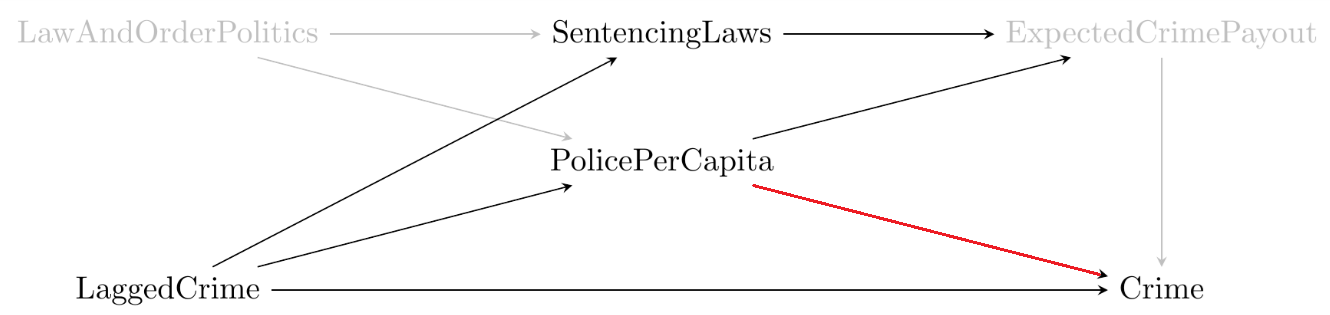
\includegraphics[width=0.7\linewidth]{24_DiDLecture/24_DiDLecture_DAG.png}
    \end{center}
    \flushright
    \tiny{ (\emph{The Effect, p.450}, Huntington-Klein)}.
\normalsize
\flushleft
    \begin{itemize}
    \item In answering a causal research question we need to account for other variables that also contribute to the the outcome in question, one way or another. 
    \item In the example DAG, without appropriate control for LaggedCrime, we could e.g. erroneously attribute higher crime rates to less PolicePerCapita.    
    \item There are many ways to accomplish this: using control variables, taking advantage of different fixed effects, randomization, using variation from a natural experiment, choosing an appropriate control group.
    \item Ultimately it depends on the question, what we need to do, but also the assumptions underlying the method we choose.
    \end{itemize}
\end{frame}


\begin{frame}{Effect heterogeneity}
\begin{itemize}
    \item The notion of a single causal effect in social science is  perhaps best described as fiction. Take the example of a new drug, while it may be very effective for some, it has no or adverse effect for others, be it because of their e.g. gender, body chemistry, or perhaps age. 
    \item This type of effect-variety is referred to as \textbf{heterogeneous treatment effects}
    \item It's possible to estimate the distribution of these effects, e.g. to predict a specific effect that pertains to an individual with certain characteristics, like in personalized medicine, often times base on \textbf{machine learning}.
    \item But in terms of estimating causal effects in social science, we are generally after some form of \textbf{average effect}. Yes there are many!
\end{itemize}
\end{frame}

\begin{frame}{Treatment-effect averages}
\begin{itemize}
    \item Having established the notion of heterogeneous treatment effects, we can easily grasp the idea of a mean effect for everyone in the population, i.e. \textbf{the average treatment effect} (ATE).
   
    \item Often times it is precisely this ATE that we would like to know: If we implement a policy on everyone, what would be it's average effect?

    \item However, it's not always possible to estimate the ATE or sometimes not even desirable. The ATE for a new treatment for testicular or breast cancer is not desirable in determining it's efficiency.

    \item In running a medical trial for the associated drug, surely the participants are limited to either women or men. In this case, the average effect instead refers to refers to the conditional ATE (CATE), which is the ATE but conditional on being either male or female.
\end{itemize}
\end{frame}

\begin{frame}{The average treatment effect of the treated (ATT)}
\begin{itemize}
      \item Because of research design (such as with DiD), we often end up estimating something else, which is the average effect for the group that gets treated, in other words the \textbf{average treatment effect of the treated} (ATT or ATET).

      \item However, should we have a large random sample there is rather likely that ATT = ATE (or CATE when it's applicable).

      \item As for the ATE. In a random control trial, when the sample is representative of the population the  effect corresponds to the ATE. If it's not representative, it's conditional on being in the sample.
\end{itemize}
\end{frame}

\begin{frame}{Difference-in-Difference: What is it?}
\begin{itemize}
        \item Difference-in-differences is a statistical method or technique popular in social science with observational data that mimics an experimental research design. 

        \item It relies on two groups; one treated and one untreated control group. In DiD, the outcome is first measured over time for each group (the first difference) and the compared against one another (second difference). The result from these two differences can be a causal estimate. 

        \item Importantly, the notion of a control group is a place holder for "our best guess at what the treatment group would have been without treatment" \tiny{ (\emph{The Effect, p.450}, Huntington-Klein)}.
\normalsize
        \item \textbf{The plan} with DiD is to use the change within some untreated control group to represent all changes within the treatment group that is not due to the treatment.
\end{itemize}
\normalsize
\end{frame}

\begin{frame}{What does the DiD results actually mean and is the effect really causal?}
        \begin{itemize}        
        \item Since out plan was to use the control group to "represent all changes \textbf{within the treatment group} that is not due to the treatment", the DiD estimate the effect for the treated group. 

        \item If certain conditions are satisfied, specifically the assumption of the so called \textbf{parallel trends}, the DiD estimate represents a well defined causal parameter, namely the average treatment effect of the treated (ATT). \textbf{This is the connection between DiD and causality.}
        
        \item For the DiD estimate, therefore, we could not know if the treatment effect would be any different for other groups!        
    \end{itemize}
\end{frame}

\begin{frame}{The history of DiD goes back more than 150 years}
    \begin{itemize}
        \item Today somewhat of a cliché, but still very instructional.
        \item In 1855, John Snow (like an Aegon Targaryen) demonstrated for the first time and for the world that cholera was spread by contaminated water and not through the air. 
        \item The culprit, water intake downstream the river Thames contained all sorts of sewage waste.
        \item Between 1849 and 1854 a policy was implemented that required the Lambeth Company move their water intake upstream outside of London. 
        \item The results...        
    \end{itemize}
\end{frame}

\begin{frame}{What happened with death rate in areas served by the Lambeth company?}
\begin{figure}[H]
\centering
        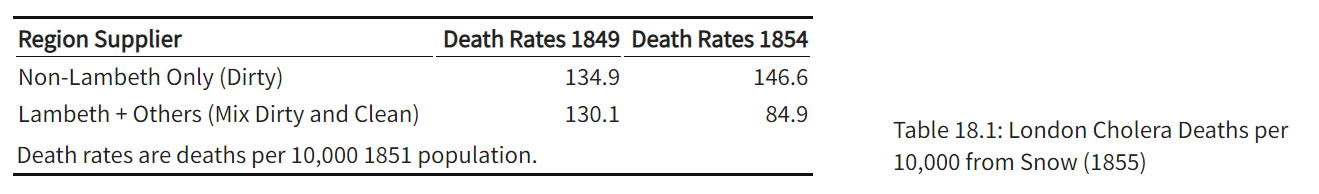
\includegraphics[width=1\linewidth]{24_DiDLecture/24_DiDLecture_John Snow.png}
    \tiny (\emph{The Effect, p.438}, Huntington-Klein)
\end{figure}

\begin{itemize}
    \item Let's compare the differences in death rates between 1854 and 1849 for Lambeth and non-Lambeth
    \item For Lambeth we get $84.9 - 130.1 = -45.2$ and for non-Lambeth $146.6 - 134.9 = 11.7$ 
    \item How much do the difference differ?  $-45.2-11.7=-57.1$
    \item By moving the water pump, the cholera mortality rate decreased by $57.1$ deaths per $10,000$. 
\end{itemize}
\end{frame}

\begin{frame}{Today Difference-in-Difference is still highly relevant}
\begin{columns}
\begin{column}{0.5\textwidth}
  \begin{itemize}
        \item At least in economics is Difference-in-Difference (or DiD) arguably the most widely used method for estimating causal effects in non-experimental settings. 
        \item An early and influential study is David Card (1990), \emph{The Impact of the Mariel boatlift on the Miami labor market}, IRL Review 43(2):245-257. 
    \end{itemize}
\end{column}

\begin{column}{0.5\textwidth}
 \begin{center}
        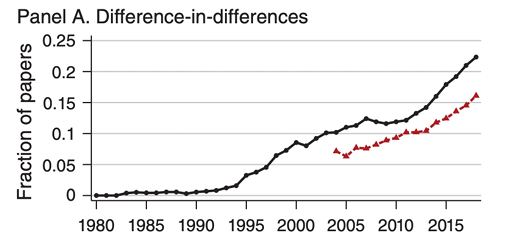
\includegraphics[width=1\linewidth]{24_DiDLecture/24_DiDLecture_AEA_DiD.png}
    \end{center}
\end{column}
\end{columns}
\end{frame}

\begin{frame}{Let's work through an example using real data}
\begin{itemize}
    \item We are going to use the data from the paper by Kessler and Roth (2014) called \emph{Don't take "no" for an answer: And experiment with actual organ donor registrations} 
    \item Most US states have so called "opt-in" (as opposed to "opt out") organ donation programs. When you get your drivers license you can choose to partake in the organ donation program.
    \item In July 2011, California implemented a policy to switch from an "opt-in" program to one with "active choice", of either yes or no. 
    \item Did the policy positively affect the donation rate \underline{in California}, as anticipated by the policy makers? 
\end{itemize}
\end{frame}

\begin{frame}{*Organ donation rates in the US}
\begin{columns}
\begin{column}{0.5\textwidth}
  
\begin{itemize}
    \item The Kessler and Roth data can be retrieved from:
\end{itemize}
\href{https://github.com/DanielHalvarsson/IntroductionDiD/}{\textcolor{blue}{https://github.com/DanielHalvarsson/\\IntroductionDiD/}}
\begin{itemize}
    \item You can download the data manually using the above link. And open the data file from within Stata.
    \item Alternatively, the data can be retrieve directly from within Stata by linking directly to the 'organ\_donations.dta' file.
    \item To follow along, you need to have the following Stata packages installed: $reghdfe$
\end{itemize}
\end{column}
\begin{column}{0.5\textwidth}
 \begin{center}
        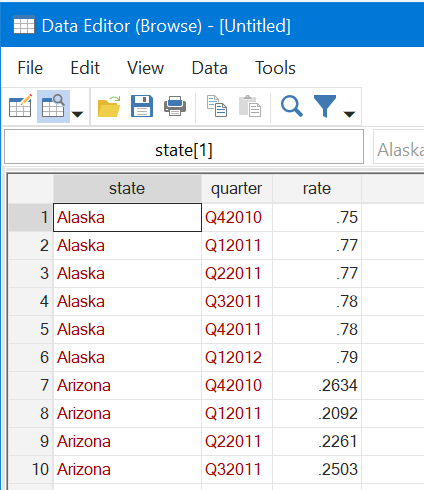
\includegraphics[width=0.7\linewidth]{24_DiDLecture/24_DiDLecture_LoadData.png}
    \end{center}
\end{column}
\end{columns}
\end{frame}

\begin{frame}{*Visualizing the organ donation rates over time}
\begin{enumerate}
    \item Lets create the following plot.
\end{enumerate}
 \begin{center}
        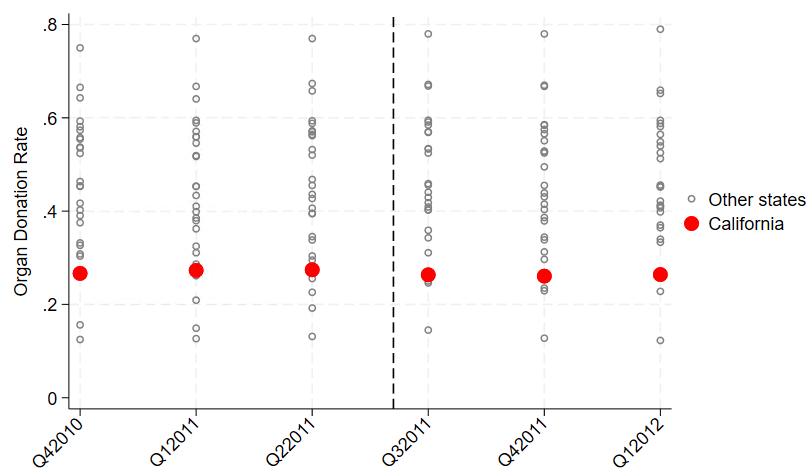
\includegraphics[width=0.7\linewidth]{24_DiDLecture/24_DiDLecture_PlotAll.png}
    \end{center}
\end{frame}

\begin{frame}{*Did the policy causally affect the donation rate 
\underline{in California}?}
\begin{columns}
\begin{column}{0.5\textwidth}
\begin{itemize}
    \item To answer that question, we calculate the $2\times2$ Difference-in-Difference.
    \item \textbf{Just like with the cholera example we are in the business of comparing averages.}
    \item The DiD effect amounts to a  \textcolor{orange}{-2.24} percentage point reduction in organ donation rates, following the policy in California.
\end{itemize}
\end{column}
\begin{column}{0.5\textwidth}
 \begin{center}
        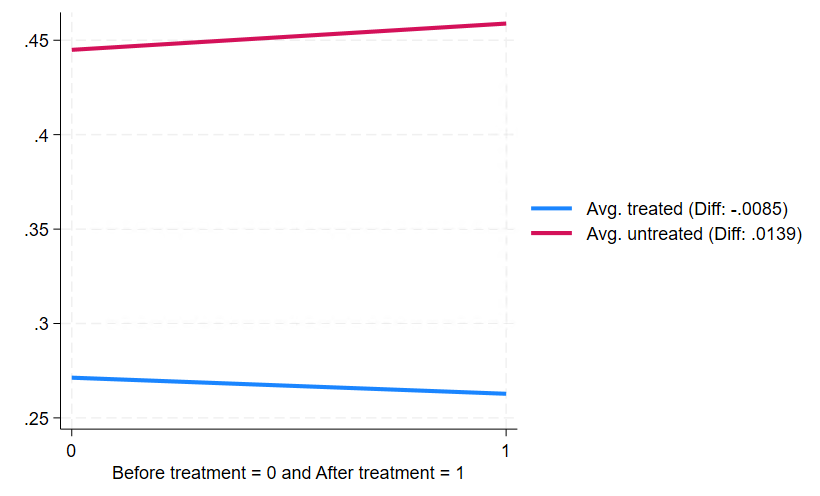
\includegraphics[width=1\linewidth]{24_DiDLecture/24_DiDLecture_DiD2x2Plot.png}
    \end{center}
\end{column}
\end{columns}
    \flushright
    \vspace{1cm}
    Difference-In-Difference estimate: $-0.0085 - 0.0139 =$   \textcolor{orange}{$ -0.0224$}
\end{frame}

\begin{frame}{Is a DiD estimate the causal ATT effect?}
\begin{itemize}
    \item It depends... 

    \item For DiD to work, we obviously need an untreated control group. Specifically, we need an untreated control group that satisfies the \textbf{parallel trends assumption}.

    \item According to the parallel trends assumption:
\end{itemize}
  \begin{displayquote}
"if no treatment had occurred, the difference between the treated group and the untreated group would have stayed the same in the post-treatment period as it was in the pre-treatment period."
\flushright\tiny (\emph{The Effect, p.441}, Huntington-Klein)
\end{displayquote}
\begin{itemize}
    \item Importantly, \textbf{the parallel trends assumption can in no way be tested} as it concerns the counterfactual, i.e. how things would have turned out, had there been no treatment.
\end{itemize}
\end{frame}

\begin{frame}{The parallel trends assumption}
\begin{itemize}
    \item Recall that the plan with DiD was to use the change in the untreated group to represent all non-treated related changes in the treated group. 
    \item To see what this means consider the difference in outcome for the treated group before and after the treatment as $TretmentEffect + OtherTreatedGroupChanges$    
    \item For the untreated group, the difference in outcome before and after the treatment is given by $OtherTreatedGroupChanges$
    \item The DiD estimate is therefore given by
\begin{equation}
TretmentEffect + OtherTreatedGroupChanges - OtherTreatedGroupChanges
\end{equation}
    \item For the DiD to identify only the treatment effect, it's required that $OtherTreatedGroupChanges = OtherTreatedGroupChanges$, precisely as stated by the parallel trends assumption!
\end{itemize}
\end{frame}

\begin{frame}{The parallel trends assumption}
\fbox{\begin{minipage}{\textwidth}
\textcolor{orange}{if no treatment had occurred, the difference between the treated group and the untreated group would have stayed the same in the post-treatment period as it was in the pre-treatment period.}    
\end{minipage}}
\vspace{0.3cm}
\begin{itemize}
    \item To unpack this equality. Let's imagine the counterfactual world where no treatment has or will ever happened. 
    \item  If the parallel trends assumption holds, then the outcome for both the treated and untreated groups should experience the same change over time.
    \item But if they experience the same change over time, it must be also the case that $OtherTreatedGroupChanges = OtherTreatedGroupChanges$.
    \item Since we don't live in the counterfactual world, we can never know whether this any of this is true.  
\end{itemize}
\end{frame}

\begin{frame}{Three good reasons for why your DiD design is believable}
\begin{itemize}
    \item Even if the parallel trends assumption can't be tested, there are goods signs to look for. 
    \end{itemize}

        \begin{enumerate}
        \item We can not think of a good reason for why the outcome in the untreated group would suddenly change at the time of treatment.
        \item The characteristics of the treated and untreated groups are generally similar.
        \item Looking at time periods leading up to the treatment date, the dependent variable evolves similarly for the treated and untreated group.   
        \end{enumerate}
        \begin{itemize}

    \item What it often times comes down to in practice is to pick a control group such that 1-3 is believable.
\end{itemize}
\end{frame}

\begin{frame}{Additional implications of the parallel trends assumption}
\begin{itemize}
    \item The parallel trends assumption is not only an assumption about causality, but also about the gap (or difference) that is supposed to remain constant.
    \item Therefore, if the parallel trends assumption holds for some '$Y$' it does not hold for transformations of '$Y$', which includes '$\log Y $'
    \item It is easy to see that if the gap before the treatment was e.g. $20-10 = 10$ and the counterfactual difference after the treatment was $25-15 = 10$, in logs we get $\ln 20 - \ln 10\approx0.3$ and $\ln 25 - \ln 15\approx0.22$. 
    \item Finally, there is a risk associated with pre-testing, as it can cause statistical problems by potentially contaminating your design.
\end{itemize}
\end{frame}

\begin{frame}{How can we check if our untreated group is appropriate?}
\begin{itemize}
\item Even if we can't test the parallel trends assumption, we can and should test for common pretrends (good sign nr. 3), \textbf{IF} we have more than two time periods.
\item The second test we can do is a \emph{placebo test}. It means that we throw out all the dates for which the treatment was in effect and pick different periods before the actual treatment to see if the same DiD analysis gives a zero effect.
\item If the placebo test would show up significant, we can count that as evidence that something can be problematic with the parallel trends assumption. 
\item However, with more than two time periods we should preferably move our DiD analysis into a regression framework.
\end{itemize}
\end{frame}

\begin{frame}{Difference-in-Difference in a regression setting}
\begin{itemize}
\item For the $2\times2$ DiD analysis with two groups and two periods, we can reach exactly the same DiD estimate by using a regression. Isn't that neat!
\item Instead of tediously comparing means, we can instead estimate the following regression model for some outcome 'Y':
\begin{align}
Y = &\beta_0 + \beta_1 AfterTreatment + \beta_2 TreatedGroup\\ \nonumber
&+ \beta_3 AfterTreatment \times TreatedGroup + \epsilon
\end{align}
\item with  $AfterTreatment$ being a dummy variable that takes the value of one the period after treatment and zero the period before treatment.
\item and where $TreatedGroup$ is a dummy variable that takes the value of one for the treated group and the and zero for the untreated group. 
\item  $AfterTreatment \times TreatedGroup$ is an interaction term that takes the value of one for the treated group after treatment, and zero otherwise.
\end{itemize}
\end{frame}

\begin{frame}{Difference-in-Difference in a regression setting}
\begin{itemize}
\item Exactly the same DiD estimate as before is here given by $\hat{\beta}_3$.
\item This is fairly easy to see. Considering the average outcomes (Y) across the four different groups: 
    \begin{itemize}
    \item $TreatedGroup=0$ and $AfterTreatment=0$ gives $Y=\beta_0$ 
    \item $TreatedGroup=0$ and $AfterTreatment=1$ gives $Y=\beta_0 + \beta_1$ 
    \item $TreatedGroup=1$ and $AfterTreatment=0$ gives $Y=\beta_0 + \beta_2$ 
    \item $TreatedGroup=1$ and $AfterTreatment=1$ gives $Y=\beta_0+\beta_1+\beta_2+\beta_3$ 
    \end{itemize}
\item Now take the difference for the untreated group after and before treatment  $\beta_0 +\beta_1 -\beta_0 = \beta_1$
\item Take the same difference but for the treated group  $\beta_0 +\beta_1 +\beta_2 + \beta_3 - \beta_0 -\beta_2= \beta_1+\beta_3$
\item To get the DiD, subtract the untreated difference from the treated difference to get $\beta_1 + \beta_3 - \beta_1 = \beta_3 = DiD$ according to the definition of DiD.  
\end{itemize}
\end{frame}

\begin{frame}{Leveraging DiD by using fixed-effects regression}
\begin{itemize} 
\item Note that a powerful way of rewriting the DiD regression given by
\begin{align}
Y = &\beta_0 + \beta_1 AfterTreatment + \beta_2 TreatedGroup\\ \nonumber
&+ \beta_3 AfterTreatment \times TreatedGroup + \epsilon.
\end{align}
\item By exploiting the fact that $TreatedGroups$ and $AfterTreatment$ can be regarded as fixed effects $\alpha_g$ and $\alpha_{t}$, we can write the same 2 × 2 DiD regression as follows 
\begin{equation}
Y = \alpha_g + \alpha_{t} + \beta_3 AfterTreatment \times TreatedGroup + \epsilon.
\end{equation}
\end{itemize}
\end{frame}

\begin{frame}{Two way fixed effect (TWFE) model }
\begin{itemize}
\item In the DiD specification with fixed effects 
\begin{equation}
Y = \alpha_g + \alpha_{t} + \beta_3 AfterTreatment \times TreatedGroup + \epsilon
\end{equation}
it is clear that DiD uses so called "within" variation to identify the effect. 
\item What ever \emph{unobservable} variation that does not change over the period for each group or time period is controlled for in the model and can not contaminate the "effect".    
\item But why stop there, if the treated and untreated groups are comprised of individual workers, firms, or states, we can shift the level of fixed effects from $\alpha_g$ to $\alpha_i$, where the index $i$ stands for individual units.  
\item This model is called the \textbf{Two Way Fixed Effects} or \textbf{TWFE model}, and is the work horse in many DiD applications.
\item Suppose that individuals are the unit of analysis $i$, then $\alpha_i$ would capture characteristics such as personality, upbringing, ability, gender to the extent they are correlated with Y.
\end{itemize}
\end{frame}

\begin{frame}{*Let's return to the Kessler and Roth data and run some regressions!}
\begin{enumerate}
\item We start by estimating 
\begin{align}\label{eq:reg}
Y = &\beta_0 + \beta_1 AfterTreatment + \beta_2 TreatedGroup\\ \nonumber 
&+ \beta_3 AfterTreatment \times TreatedGroup + \epsilon.  
\end{align}
\item Verify the that the coefficients corresponds to the different group means. 
 \begin{itemize}
    \item $TreatedGroup=0$ and $AfterTreatment=0$ gives $Y=\beta_0$ 
    \item $TreatedGroup=0$ and $AfterTreatment=1$ gives $Y=\beta_0 + \beta_1$ 
    \item $TreatedGroup=1$ and $AfterTreatment=0$ gives $Y=\beta_0 + \beta_2$ 
    \item $TreatedGroup=1$ and $AfterTreatment=1$ gives $Y=\beta_0+\beta_1+\beta_2+\beta_3$ 
    \end{itemize}
\item We also estimate the fixed-effects version of the regression in (\ref{eq:reg}).
\begin{equation}
Y = \alpha_g + \alpha_{t} + \beta_3 AfterTreatment \times TreatedGroup + \epsilon.
\end{equation}
\item and it's extension
\begin{equation}
Y = \alpha_i + \alpha_{t} + \beta_3 AfterTreatment \times TreatedGroup + \epsilon.
\end{equation}
\end{enumerate}
\end{frame}

\begin{frame}{*Are the DiD design supportive of the parallel trends assumption?}
    \begin{itemize}
\item With more than two periods in the data, we can have a look at pretrends and run placebo tests. Up until now we have considered only two periods by aggregating quarterly data. 
\item When testing the robustness of the DiD design, we make use of information from separate quarters. Later we will fully exploit all data in the analysis when we look at DiD with dynamic treatment effects.

\begin{enumerate}
    \item Let's plot the pretrends
    \item Test for diverging pretrends. Specifically, we estimate the model with possibly different linear time trends before treatment. 
    \begin{equation}
    Y = \alpha_g + \beta_1 TimePeriods +\beta_2 TimePeriods\times TreatmentGroup + \epsilon 
    \end{equation}
    where $TimePeriods$ is a count variable for the periods leading up to the treatmentperiod. In the model $\beta_1$ is the slope estimate of the pretrend for untreated group. For the treated group the slope estimate for the pretrend is given by  $\beta_1 + \beta_2$.\\
    \vspace{0.2cm}
    Thus, if we can't reject $H_0$ that $\beta_2=0$, then we we can draw the conclusion that the best linear approximation of the average pretrends for the treated and untreated groups are probably the same.
\end{enumerate}
\end{itemize}
\end{frame}

\begin{frame}{Are the DiD design supportive of the parallel trends assumption?}
    \begin{center}
        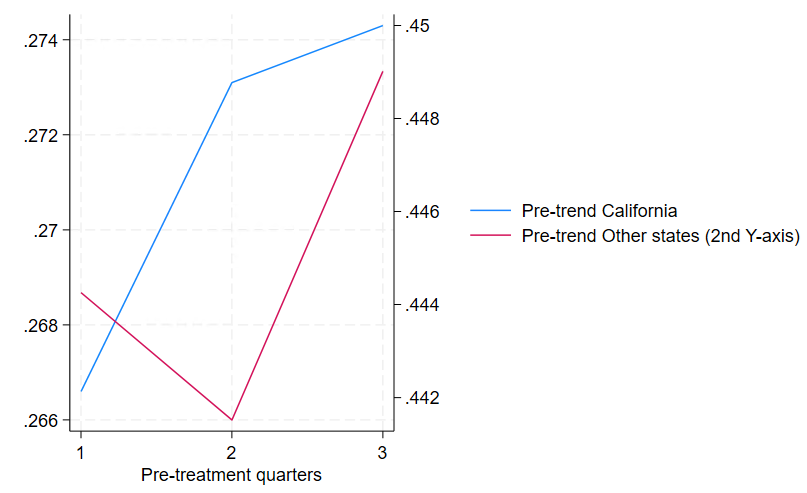
\includegraphics[width=0.55\linewidth]{24_DiDLecture/24_DiDLecture_PreTrend.png}
    \end{center}
\begin{enumerate}
  \setcounter{enumi}{2}    
    \item We also run two placebo tests. Instead of using 2011Q3 as the treatment date, we reestimate the models pretending that treatment occured 2011Q1 and 2011Q2 using data only up until 2011Q2.
\end{enumerate}
\end{frame}

\begin{frame}{What to do when the parallel assumption is likely violated?}
   \begin{itemize}
       \item In the basic DiD setting, you generally wont fix a violation in the parallel trends assumption by adding a bunch of covariates.
       \item Why?
       \item Because time invariant covariates are already controlled for by the fixed effect version of the DiD.
       \item Adding time-varying covariates can incidentally destroy identification if they themselves are caused by the treatment.
       \item A common approach is to instead look for a better control group by using some form of \textbf{statistical matching}, e.g. propensity score matching.
       \item If matching is successful, there is a good chance that the parallel trends assumption is more likely to hold.
       \item In this course, I have not chosen to further pursue matching, which is vast topic on it's own.
   \end{itemize}
\end{frame}

\begin{frame}{Dynamic DiD and long-term effects}
    \begin{itemize}
        \item So far, even with access to multiple periods, we have lumped the periods together in the period before and after treatment
        \item However, by only looking at one potential effect, useful information about how the effect changes over time may be lost.
        \item For example, it may take some time for an effect to materialize or it may taper off. 
        \item Starting from the fixed effect DiD regression, the dynamic version replaces the $AfterTreatment$ dummy in the interaction term with separate dummies for each year, both before and after treatment. 
        \item For example, a design with six periods and treatment in period four, the dynamic DiD can be written as,
        \begin{equation}
            Y = \alpha_i + \alpha_{t} + \left(\beta_{1}D_{-3}+\beta_{2} D_{-2} +\beta_{3} D_{0} + \beta_{4} D_{1}+ \beta_{5} D_{2} + \beta_{6} D_{3} \right) \times AfterTreatment + \epsilon.
        \end{equation}
        \item Often times, calender time is replaced with relative-treatment time.
    \end{itemize}
\end{frame}

\begin{frame}{*Let's code the dynamic DiD}
    \begin{enumerate}
        \item Using the organ donation data, let's code the dynamic version of the DiD.
        \item What is the interpretation?
    \end{enumerate}
    \vspace{1cm}
    \begin{center}
        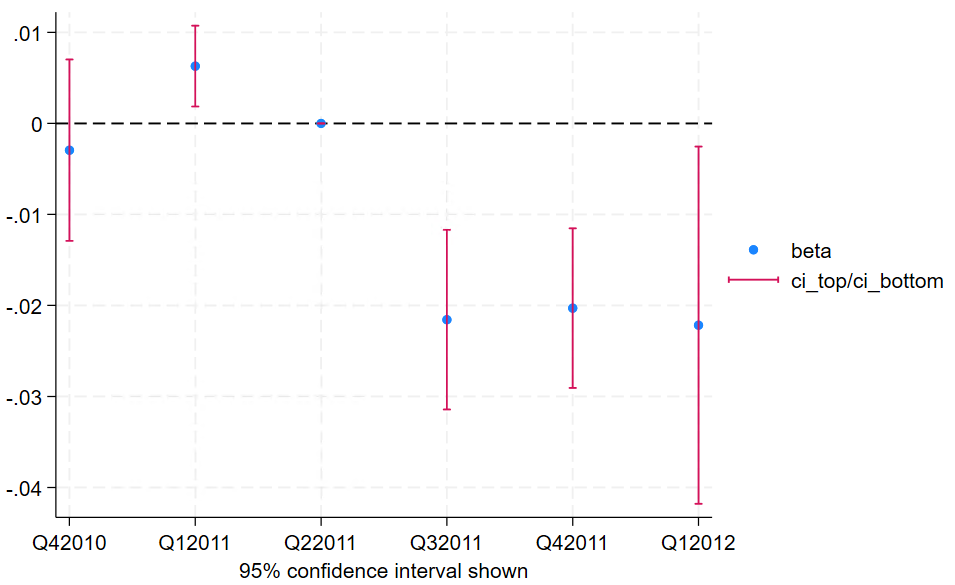
\includegraphics[width=0.6\linewidth]{24_DiDLecture/24_DiDLecture_DynamicDiD.png}
    \end{center}
\end{frame}

\begin{frame}{Interpreting the dynamic DiD results}
\begin{itemize}
\item Near zero effects during the pretreatment period (compared to Q22011)
\item One badly behaving pre-treatment effect.
\item Yet, three distinct negative effects immediately following the policy.
\item In accordance with the $2\times2$ DiD design, the dynamic DiD finds a -2.2 percentage point decrease in organ donation rates in California as a result of active choice.
\end{itemize}
\end{frame}


\begin{frame}{Insights from the dynamic specification}
\begin{itemize}
\item In addition to the additional insights that about treatment-effect dynamics
\item The dynamic DiD provides a direct test for parallel \textbf{pre}trends (a type of placebo test).
\item For each of the pretreatment gaps, they should not be larger or smaller compared to the gap before the treatment takes place, i.e. the reference.
\item With many pre-periods, however, there can be significant effects due to pure chance. Thus, the one badly behaved estimate does not necessarily imply the end of the world!
\end{itemize}
\end{frame}

\begin{frame}{Insights from the dynamic specification cont.} 
\begin{itemize}
\item However, as three are less data devoted to estimating each of the effects, expect less precise estimate.
\item Even if the individual effects is significant, the average overall effect can still be significant!  
\item Lastly, while the dynamic specification is a powerful tool when there are one treated group, it can no longer be trusted when there are many treated groups with varying treatment timing.
\end{itemize}
\end{frame}

\begin{frame}{Roll-out adoption (staggered treatment) design}
      \begin{wideitemize}
          \item Expands the dynamic DiD designs to allow for \textit{multiple groups} with \textit{different treatment adoption dates}. \item Example is a policy with a regional roll-out such that the policy is adopted in different areas at different dates.
\vspace{1cm}
    \begin{center}
        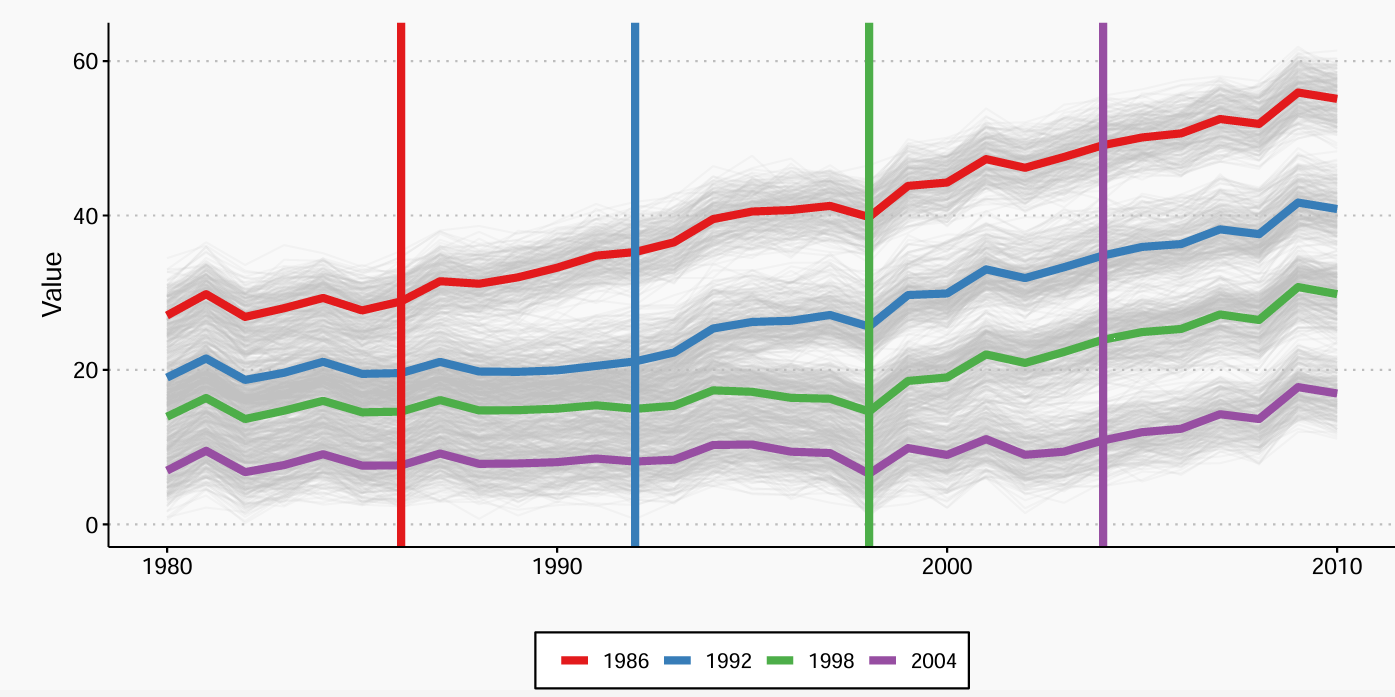
\includegraphics[width=0.6\linewidth]{24_DiDLecture/24_DiDLecture_StaggeredRollout.png}
    \end{center}
          
      \end{wideitemize}
\end{frame}

\begin{frame}{The problem with TWFE and "the secrete shame of econometrics"}
\begin{columns}[T] % align columns
    \begin{column}{0.6\textwidth}
      \begin{wideitemize} 
        \item The TWFE model is well understood and commonly applied to the basic $2\times2$ setup and to the dynamic (event-study) setup.
        \item However, for a roll-out treatment design, with different groups getting treated at different times, the TWFE model no longer works.
        \item \textbf{The problem} can be quite serious. With DiD estimates displaying a negative average effect despite the true effect being positive for everyone in the sample. 
            \end{wideitemize}
    \end{column}%
    \hfill%
    \begin{column}{.4\textwidth}
    \begin{center}
 \includegraphics[width=0.65\linewidth]{24_DiDLecture/24_DiDLecture_GoT.png}                 
    \end{center}
    \end{column}
  \end{columns}
  \begin{displayquote}
  "For decades researchers were basically unaware of this problem and used two-way fixed effects anyway."
  \flushright\tiny (\emph{The Effect, p.458}, Huntington-Klein)
\end{displayquote}
    \end{frame}

\begin{frame}{The problem}
      \begin{wideitemize}
        \item The problem is somewhat complex. 
        \item TWFE relies on \textbf{within variation} for comparing treated and controls. It means that units that \textit{remains untreated} during the period end up as controls, but the same goes for units that \textit{remains treated} from earlier roll-outs.
        \item \textbf{IF} treatment effect varies with treatment time e.g. effects grow larger over time, earlier treated units in the control group will have an increasing trend that is distinct from just-now-treated units, 
        \item \textbf{THEN} parallel trends assumption breaks and identification fails.  
        \end{wideitemize}
        \end{frame}

\begin{frame}{The State of the DiD literature}
      \begin{wideitemize}
      \item Things are moving fast 

      \item This literature has had a certain amount of upheaval over the past 5-6 years. 
        
      \item With the upheaval there is a \textbf{tension} for how people currently and historically have used DiD.

      \item The modern literature has pointed out many issues but has provided solutions to almost all of the them.
      
      \item Good tools are now readily available (including Stata), so nothing to prevent you from using a DiD with staggered analysis.
      \end{wideitemize}
\end{frame}

\begin{frame}{When TWFE is NOT a problem in staggered adoption design}
      \begin{wideitemize}
         \item However, despite the severity of the problem, as emphasized at the beginning, there are situations where TWFE estimates is reliable.
      
         \item If the treatment effect is the same across all treated groups over time the dynamic TWFE works just fine. 

         \item However, we can never know whether this is true by only estimating the dynamic TWFE model.
        \end{wideitemize}
\end{frame}

\begin{frame}{Roll-out design as many different sub-experiments}
      \begin{wideitemize}
          \item For each treated group in a roll-out design, the causal effect is just the same as in dynamic DiD when compared to an untreated group.
          \item Plenty of causal effect estimates: What to do with them? 
         \begin{wideitemize}
          \item In a small design, it could be be beneficial to analyze each of the sub-experiments separately to gain insight into treatment effect heterogeneity, although it may be statistically inefficient.
          \item In a larger study, a separate analysis may not simply be feasible (nor desirable). 
          \end{wideitemize} 
          \item For both cases it's often desirable to average or aggregate many estimates into a single causal effect.  
          \item But for this purpose, the TWFE model don't correspond to a causal effect, without imposing strong and quite artificial assumptions.
          
      \end{wideitemize}
\end{frame}

\begin{frame}{What to do with staggered timing in DiD?}

  \begin{center}
      "What to do then, when we have a nice roll-out design? Don't use two-way fixed effects, but also don't despair. \textbf{You're not out of luck, you're just moving into the realm of what the pros do}."  \tiny (\emph{The Effect, p.460}, Huntington-Klein)
  \end{center}
  
  \begin{itemize}
  \item There's really no reason to use the baseline TWFE in staggered timings
    \item TWFE is a perfect example wherein the estimator does not generate an
      estimate that maps to a meaningful estimand such as the ATT.

  \item There are different approaches proposed in the literature that are just as good.
    \item Let's have a loo at Sun and Abraham (2020), which extends the dynamic DiD model to account for the different treatment effects for different groups.     
    \end{itemize}
\end{frame}

\begin{frame}{Modified event-study design: Sun and Abraham, 2020}
\begin{wideitemize}
    \item Starting from the basic event-study design, it can be modified to include many groups with a staggered roll-out.
    \item First, each of the sub-experiments are \textbf{centered} relative to their own treatment start.
    
    \begin{itemize}
        \item It keeps track on the already treated groups so that they don't get included in comparisons.
    \end{itemize}
    
    \item Second, Sun and Abraham then propose that the relative time dummies are \textbf{interacted} with group dummies such that each treated $TreatedGroup_k\times RelativeTimeDummy$ get their own effect. 
    
    \item It's then up to you to avoid making bad comparisons when averaging coefficients to get ATT (see example below).

    \item Each effect is either compared to the group of (i) never treated observation or (ii) not yet treated observations (from the last treated group(s)).
\end{wideitemize}
\end{frame}

\begin{frame}{*Modified event-study design: Sun and Abraham, 2020}
\begin{itemize}
    \item Sun and Abraham (2020) can be accessed in Stata using the \textbf{eventstudyintereact} package.
\end{itemize}
\begin{enumerate}
    \item Let's try it out for data over female wages and union memberships.\\
  We load the nlswork.dta data from  \href{https://github.com/DanielHalvarsson/IntroductionDiD/}{\textcolor{blue}{https://github.com/DanielHalvarsson/IntroductionDiD/}}
\end{enumerate}
\vspace{0.5cm}
    \begin{center}
        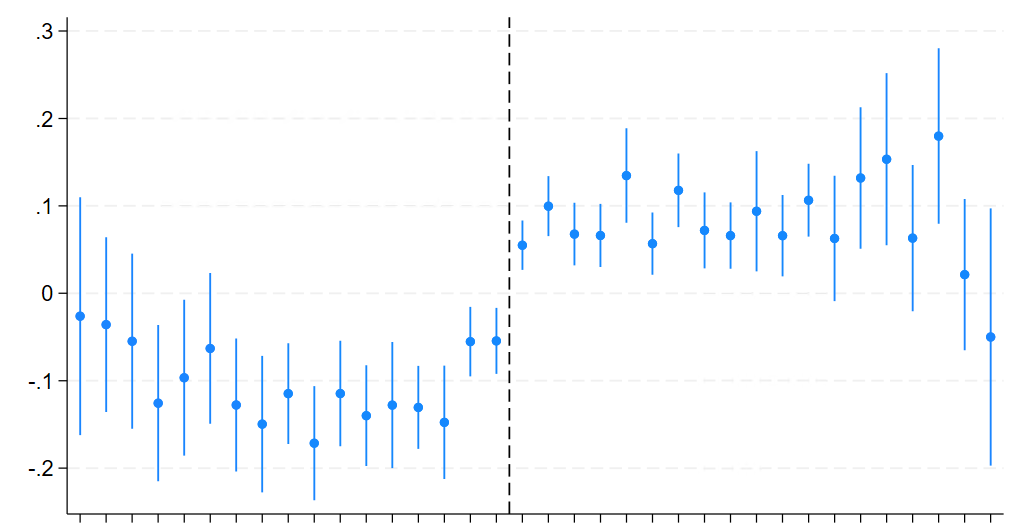
\includegraphics[width=0.6\linewidth]{24_DiDLecture/24_DiDLecture_SunAndAbraham.png}
    \end{center} 
\end{frame}

\begin{frame}{*Interpreting the results from the union application}
\begin{itemize}
    \item The gap between treated and untreated in the pretreatment period is smaller compared to the gap in the period before treatment.
    \item Why?
    \item Possibly because the gap suddenly increases just before becoming union member.
    \item It's difficult to speculate without looking closer at the data, but the pattern would agree with a situation where wages in the treated group shoots up the year before the join the union.
    \item Regardless if this is the case, it would be difficult to convince someone that the parallel trends assumption is satisfied.
\end{itemize}
\end{frame}



\begin{frame}{What's next}
\begin{itemize}
    \item Three excellent resources further study about all things difference-in-difference and other techniques, e.g. three excellent books: \textbf{The Effect} by Nick Huntington-Klein, \textbf{Causal Inference: A mixed tape} by Scott Cunningham, both of which are modern and slightly more accessible than \textbf{Mostly Harmless Econometrics} by Joshua Angrist and Jörn-Steffen Pischke.
    \item There are also excellent survey papers covering many recent contributions to the field, including techniques suitable for roll-out design: \textbf{What’s trending in difference-in-differences? A synthesis of the recent econometrics literature} by Jonathan Roth, Pedro H.C. Sant’Anna, Alyssa Bilinski and John Poe, and \textbf{Designing difference in difference studies with staggered treatment adoption: key concepts and practical guidelines} by Seth Freedman, Alex Hollingsworth, Kosali Simon, Coady Wing, ad Madeline Yozwiak. 
\end{itemize}
\end{frame}

\begin{frame}{\centering Thank you!}
\begin{itemize}
\item Ýou find a home assignment on \href{https://github.com/DanielHalvarsson/IntroductionDiD/}{\textcolor{blue}{https://github.com/DanielHalvarsson/IntroductionDiD/}}
\item Next time we meet on November 25, we'll go through it. 
\item In the mean time, if you have questions, my email is \href{daniel.halvarsson@ratio.se}{\textcolor{blue}{daniel.halvarsson@ratio.se}}
\item Good luck!
\end{itemize}

\end{frame}

\end{document}

